\subsection{Torque control, an alternative reaction wheel controller}

An alternative, torque motor controller was implemented in the simulation environment. Since the torque control is done through current control, the dynamics time constant is rather small, thus the simulation became quite computation demanding. For controlling the current, the motor inductance needs to be taken into account. Even though torque control is more appropriate than angular velocity control, since it does not have torque delay, the simulations proved that the angular velocity controller can track the torque demand sufficiently. This is due to the fact that the satellite does not require sudden high speed attitude changes.

The torque control scheme works as follows: the main attitude controller sends a torque demand to the actuators, which is then distributed between the actuators. Each of the reaction wheels get their own individual torque demand signals. Two methods have been implemented for tracking this torque demand. One is by transforming the torque to angular velocity demand, which the motor has to track, the other is directly controlling for actuator error.

\begin{figure}[h!]
	\centering 
	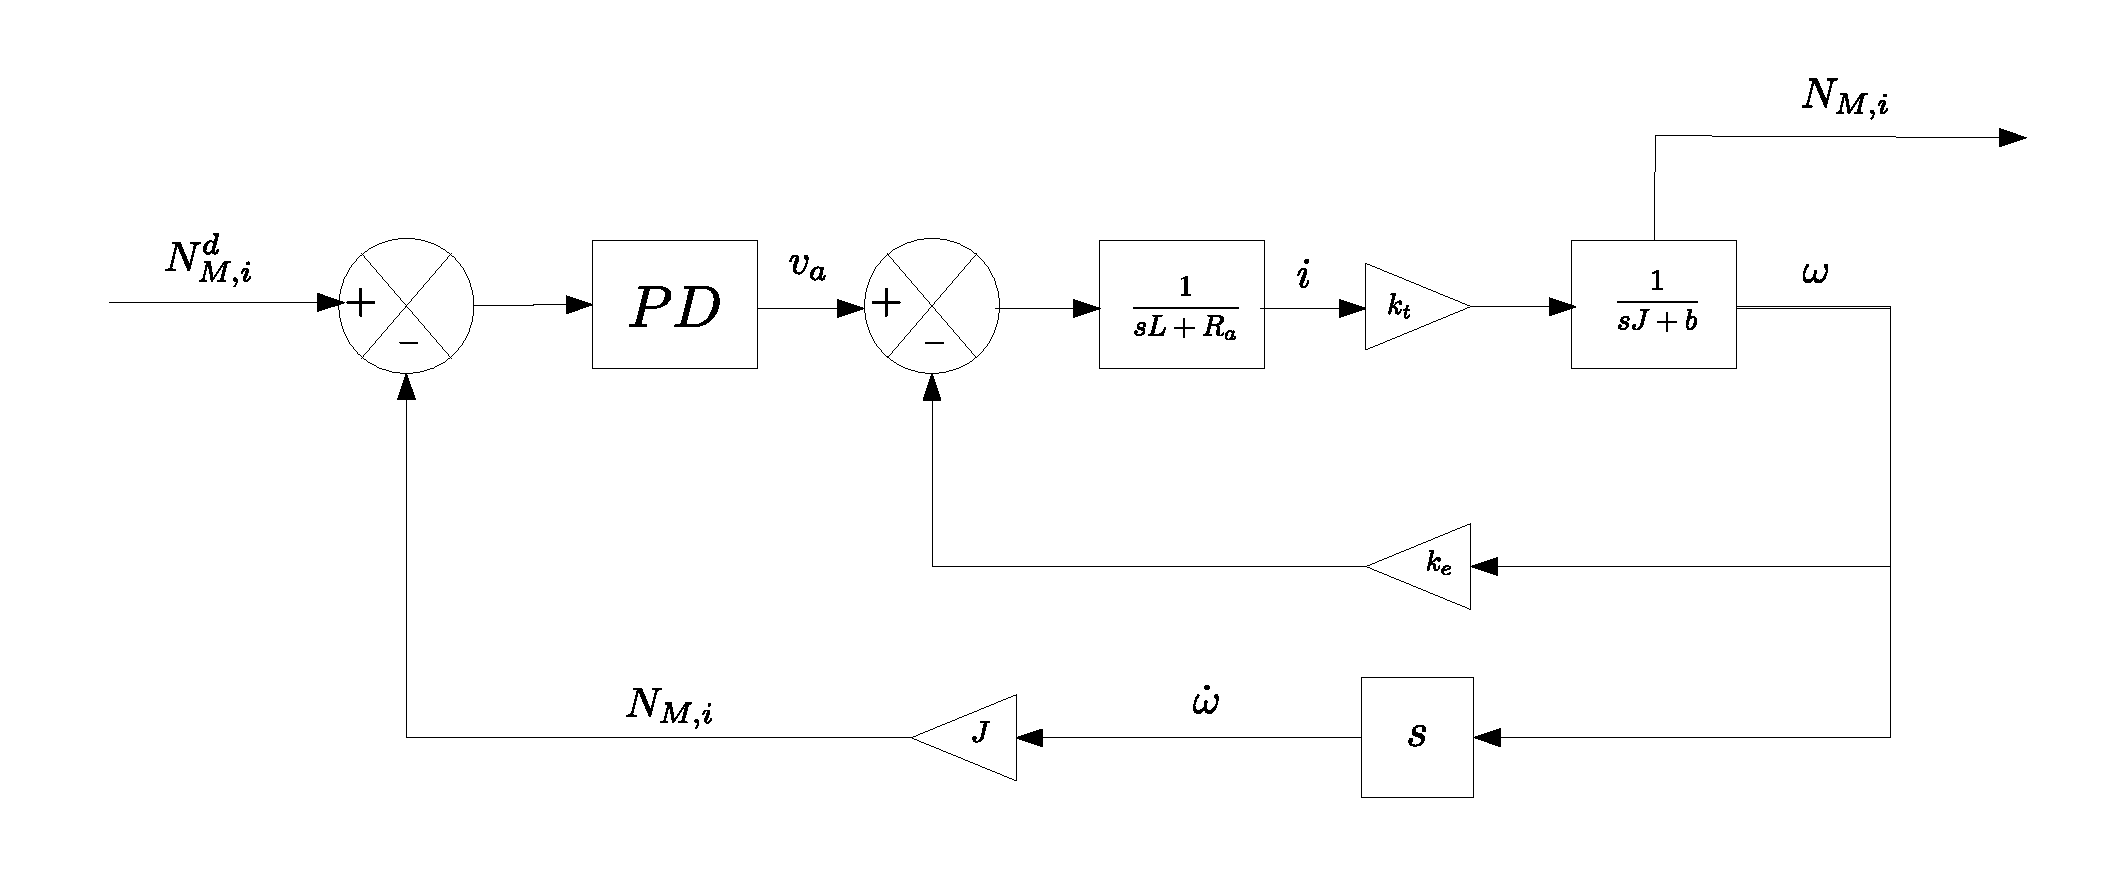
\includegraphics[width=170mm]{figures/torqueControl.pdf}	
	\caption{Torque control scheme.}
	\label{fig:torqueControl}
\end{figure}

As shown on Figure \ref{fig:torqueControl} , the torque controller controls the torque error signal using a PD controller. Since the torque has a $ 10^{-5} Nm$ magnitude, while the voltage has $ 10^1 V$, numerically the PD gains are quite large. The control signal is the input voltage for the DC motor. The subsystem is second order, including an integrator for current and one for angular velocity.
